\documentclass[border=6pt]{standalone}
\usepackage{tikz}
\usetikzlibrary{arrows.meta,positioning,calc,shapes.geometric}
\begin{document}
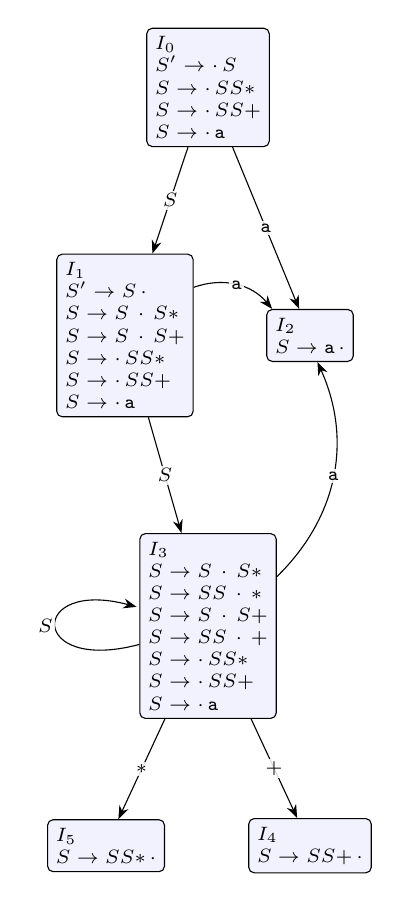
\begin{tikzpicture}[>=Stealth,font=\scriptsize,x=1.000cm,y=1.000cm,
 box/.style={draw,rounded corners=2pt,align=left,inner sep=3pt,fill=blue!5},
 circ/.style={draw,circle,align=center,inner sep=1pt,minimum size=0.75cm,fill=blue!5},
 lab/.style={font=\scriptsize,inner sep=1pt,fill=white,fill opacity=0.85,text opacity=1}]
\node[box] (s0) at (0.000,0.000) {\textbf{$I_{0}$}\\$S' \to \cdot\,S$\\$S \to \cdot\,S S \mathtt{*}$\\$S \to \cdot\,S S \mathtt{+}$\\$S \to \cdot\,\mathtt{a}$};
\node[box] (s1) at (-1.055,-3.150) {\textbf{$I_{1}$}\\$S' \to S\,\cdot$\\$S \to S\,\cdot\,S \mathtt{*}$\\$S \to S\,\cdot\,S \mathtt{+}$\\$S \to \cdot\,S S \mathtt{*}$\\$S \to \cdot\,S S \mathtt{+}$\\$S \to \cdot\,\mathtt{a}$};
\node[box] (s2) at (1.295,-3.150) {\textbf{$I_{2}$}\\$S \to \mathtt{a}\,\cdot$};
\node[box] (s3) at (0.000,-6.840) {\textbf{$I_{3}$}\\$S \to S\,\cdot\,S \mathtt{*}$\\$S \to S S\,\cdot\,\mathtt{*}$\\$S \to S\,\cdot\,S \mathtt{+}$\\$S \to S S\,\cdot\,\mathtt{+}$\\$S \to \cdot\,S S \mathtt{*}$\\$S \to \cdot\,S S \mathtt{+}$\\$S \to \cdot\,\mathtt{a}$};
\node[box] (s4) at (-1.295,-9.630) {\textbf{$I_{5}$}\\$S \to S S \mathtt{*}\,\cdot$};
\node[box] (s5) at (1.295,-9.630) {\textbf{$I_{4}$}\\$S \to S S \mathtt{+}\,\cdot$};
\draw[->] (s0) -- node[lab,midway] {$S$} (s1);
\draw[->] (s0) -- node[lab,midway] {$\mathtt{a}$} (s2);
\draw[->] (s1) -- node[lab,midway] {$S$} (s3);
\draw[->] (s1) to[bend left=35] node[lab,midway] {$\mathtt{a}$} (s2);
\path[->] (s3) edge[loop left] node[lab] {$S$} (s3);
\draw[->] (s3) -- node[lab,midway] {$\mathtt{*}$} (s4);
\draw[->] (s3) -- node[lab,midway] {$\mathtt{+}$} (s5);
\draw[->] (s3) to[bend right=35] node[lab,midway] {$\mathtt{a}$} (s2);
\end{tikzpicture}
\end{document}
